\documentclass[12pt]{exam}

% essential packages
\usepackage{fullpage} % margin formatting
\usepackage{enumitem} % configure enumerate and itemize
\usepackage{amsmath, amsfonts, amssymb, mathtools} % math symbols
\usepackage{xcolor, colortbl} % colors, including in tables
\usepackage{makecell} % thicker \Xhline in table
\usepackage{graphicx} % images, resizing

% sometimes needed packages
\usepackage{hyperref} % hyperlinks
\usepackage{tikz} % drawing graphs
\usetikzlibrary{positioning}

% paragraph formatting
\setlength{\parskip}{6pt}
\setlength{\parindent}{0cm}

% newline after Solution:
\renewcommand{\solutiontitle}{\noindent\textbf{Solution:}\par\noindent}

% less space before itemize/enumerate
\setlist{topsep=0pt}

% creates \filcl to grey out cells for groupwork grading
\newcommand{\filcl}{\cellcolor{gray!25}}

% creates \probnum to get the problem number
\newcounter{probnumcount}
\setcounter{probnumcount}{1}
\newcommand{\probnum}{\arabic{probnumcount}. \addtocounter{probnumcount}{1}}

% use roman numerals by default
\setlist[enumerate]{label={(\roman*)}}

% creates custom list environments for grading guidelines, question parts
\newlist{guidelines}{itemize}{1}
\setlist[guidelines]{label={}, left=0pt .. \parindent, nosep}
\newlist{gwguidelines}{enumerate}{1}
\setlist[gwguidelines]{label={(\roman*)}, nosep}
\newlist{qparts}{enumerate}{2}
\setlist[qparts]{label={(\alph*)}}
\newlist{qsubparts}{enumerate}{2}
\setlist[qsubparts]{label={(\roman*)}}
\newlist{stmts}{enumerate}{1}
\setlist[stmts]{label={(\roman*)}, nosep}
\newlist{pflist}{itemize}{4}
\setlist[pflist]{label={$\bullet$}, nosep}
\newlist{enumpflist}{enumerate}{4}
\setlist[enumpflist]{label={(\arabic*)}, nosep}

\printanswers

\newcommand{\prevhwnum}{7}
\newcommand{\hwnum}{8}

\begin{document}
%%%%%%%%%%%%%%% TITLE PAGE %%%%%%%%%%%%%%%
\title{EECS 203: Discrete Mathematics\\
  Winter 2024\\
  Homework \hwnum{}}
\date{}
\author{}
\maketitle
\vspace{-50pt}
\begin{center}
  \huge Due \textbf{Thursday, April 4}, 10:00 pm\\
\Large No late homework accepted past midnight.\\
\vspace{10pt}
\large Number of Problems: $8+2$
\hspace{3cm}
Total Points: $100+30$
\end{center}
\vspace{25pt}
\begin{itemize}
    \item \textbf{Match your pages!} Your submission time is when you upload the file, so the time you take to match pages doesn't count against you.
    \item Submit this assignment (and any regrade requests later) on Gradescope. 
    \item Justify your answers and show your work (unless a question says otherwise).
    \item By submitting this homework, you agree that you are in compliance with the Engineering Honor Code and the Course Policies for 203, and that you are submitting your own work.
    \item Check the syllabus for full details.
\end{itemize}
\newpage
%%%%%%%%%%%%%%% TITLE PAGE %%%%%%%%%%%%%%% 

\section*{Individual Portion}

\subsection*{\probnum Easy Peasy Degree-sy Squeezy [8 points]}
Let $G$ be a graph with $v$ vertices and $e$ edges. Let $M$ be the maximum degree of the vertices of $G$, and let $m$ be the minimum degree of the vertices of $G$. Show that
\begin{qparts}
    \item $\dfrac{2e}{v} \geq m$
    \item $\dfrac{2e}{v} \leq M$
\end{qparts}

\begin{solution}
    \begin{qparts}
        \item The total degree of the vertices is $2e$, since each edge is counted twice by its two vertices. 
        \par Let every vertex have $2e$ "vacancies," that is, spots for edges to fill. (Essentially, for each vertex, this "vacancy" number is just the difference between $2e$ and the degree of that vertex.) Then there will be $2ev$ "vacancies" total among the vertices, before edges fill them. After subtracting the edges, there will be $2ev - 2e$ total "vacancies" left among the edges. Let the pigeons be the "vacancies" and the vertices be the holes. Then by the Pigeonhole Principle, there must be at least one vertex with at least $\frac{2ev - 2e}{v} = 2e - \frac{2e}{v}$ ``vacancies.'' This translates to a degree of $2e - \left(2e - \frac{2e}{v}\right) = \frac{2e}{v}$. So there is at least one vertex with degree at most $\frac{2e}{v}$. Since the minimum degree must be less than or equal to this, $\dfrac{2e}{v} \geq m$.
        \item The total degree of the vertices is $2e$, since each edge is counted twice by its two vertices. There are $v$ vertices (holes) and $2e$ total degree (pigeons). So by the pigeonhole principle, there is one vertex with degree at least $\dfrac{2e}{v}$. Since the maximum degree must be greater than or equal to this degree, $\dfrac{2e}{v} \leq M$.
    \end{qparts}
\end{solution}

\clearpage

\subsection*{\probnum The Forest Beyond the Trees [15 points]}
Determine which of the following graphs is/are a tree. Additionally, determine which of the following graphs is/are bipartite. Please explain your reasoning for why each one is or is not a tree, and why each one is or is not bipartite.
\begin{qparts}
    \item $C_4,$ a cycle of length 4
    \item ~\\
    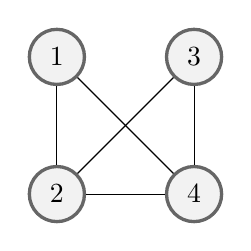
\begin{tikzpicture}[
    roundnode/.style={circle, draw=black!60, fill=gray!10, very thick, minimum size=7mm},
    ]
    %Nodes
    \node[roundnode] (1) {1};
    \node[roundnode] (2) [below=of 1] {2};
    \node[roundnode] (3) [right=of 1] {3};
    \node[roundnode] (4) [below=of 3] {4};
    
    \draw[-] (3)--(4);
    \draw[-] (2)--(3);
    \draw[-] (4)--(2);
    \draw[-] (2)--(1);
    \draw[-] (1)--(4);
    \end{tikzpicture}

    \item $K_6$
    \item ~\\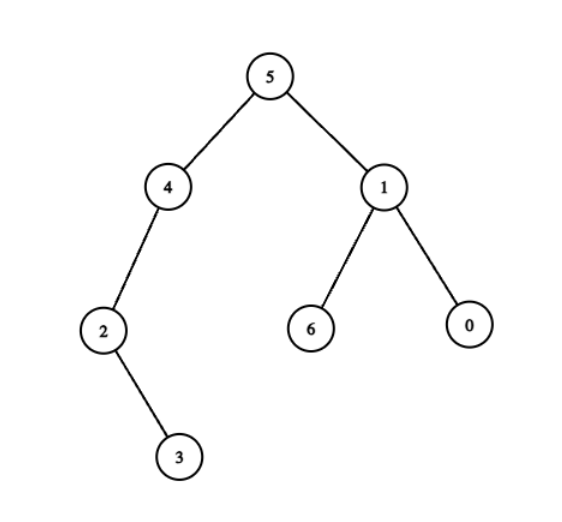
\includegraphics[scale = 0.8]{images/08-2d.png}
    \item ~\\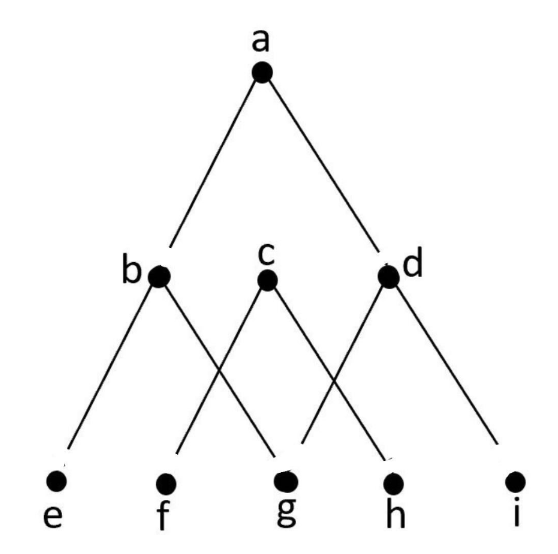
\includegraphics[scale = 0.8]{images/08-2e.png}
\end{qparts}

\begin{solution}
    \begin{qparts}
        \item This is not a tree since it contains a cycle subgraph. However, it is bipartite since it doesn't have a odd cycle.
        \item This is not a tree since it contains cycle subgraphs (e.g. the cycle of nodes 1-2-4). Additionally, it is not bipartite since it contains odd cycles. (e.g. the cycle of nodes 1-2-4).
        \item This is not a tree since it contains many cycle subgraphs. It is also not bipartite since it contains odd cycles. (Since it is complete, there is a cycle between any set of vertices, e.g. vertices 1, 2, 3)
        \item This is a tree because it contains no cycles. Additionally, 
        \item ~\\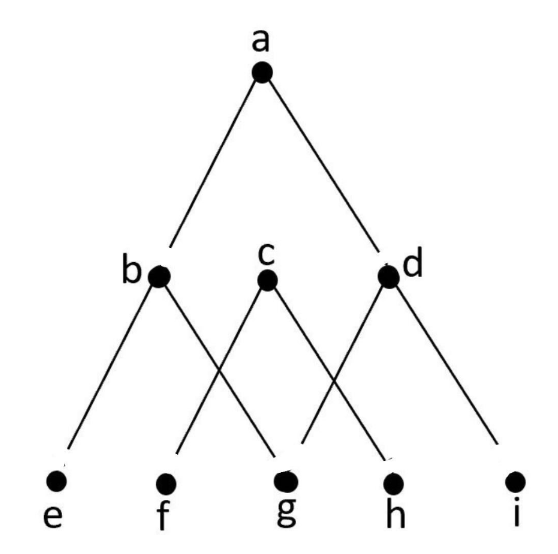
\includegraphics[scale = 0.8]{images/08-2e.png}
    \end{qparts}
\end{solution}

\newpage
\subsection*{\probnum Road Rage [12 points]}
The graphs below shows some major roads in New Jersey. The graph on the left shows distances between cities on these roads, and the graph on the right shows the toll costs on each road.

\resizebox{\textwidth}{!}{
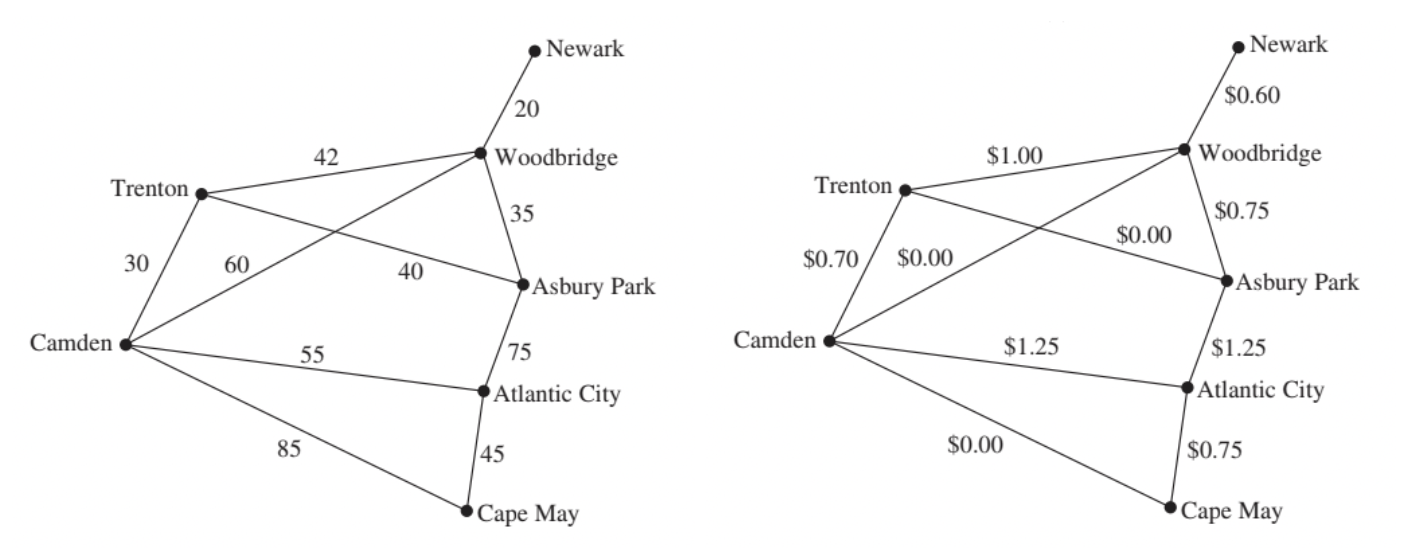
\includegraphics[]{images/08-3.png}
}

For each pair of cities below, (i) find the shortest path in distance, and (ii) find the least expensive route (shortest path in terms of cost). Be sure to list the total distance and total cost for each respective part.

\begin{qparts}
    \item Newark to Camden
    \item Trenton to Atlantic City
\end{qparts}

\begin{solution}
\end{solution}

\newpage
\subsection*{\probnum Isomorphish? [12 points]}
Determine whether or not each of the following pairs of graphs are isomorphic. If yes, provide an isomorphism. If not, explain why and propose a change to one of the graphs that would make them isomorphic; you do not need to provide an isomorphism in this case.
\begin{qparts}
    \item ~\\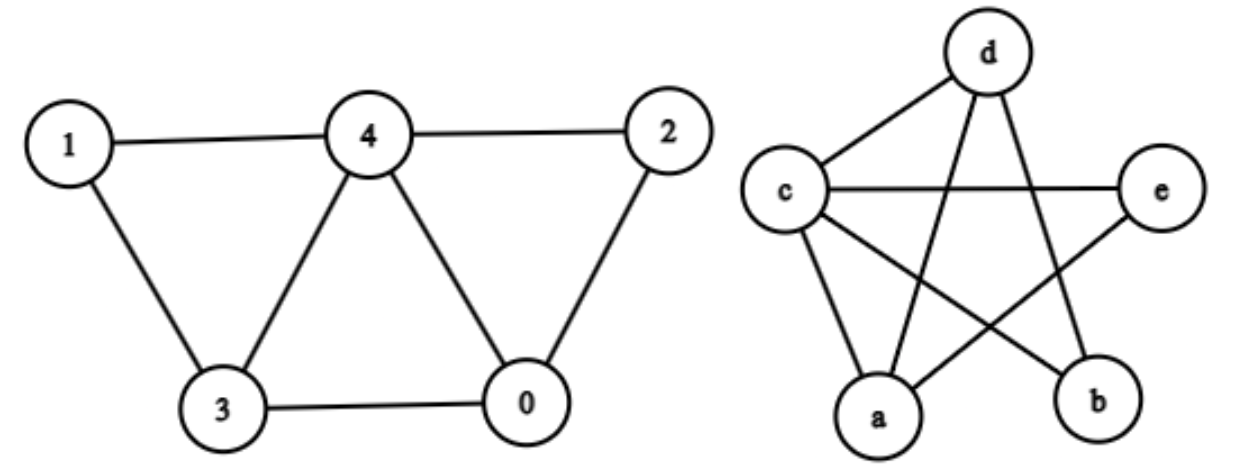
\includegraphics[width=14cm]{images/08-4a.png}
    \item ~\\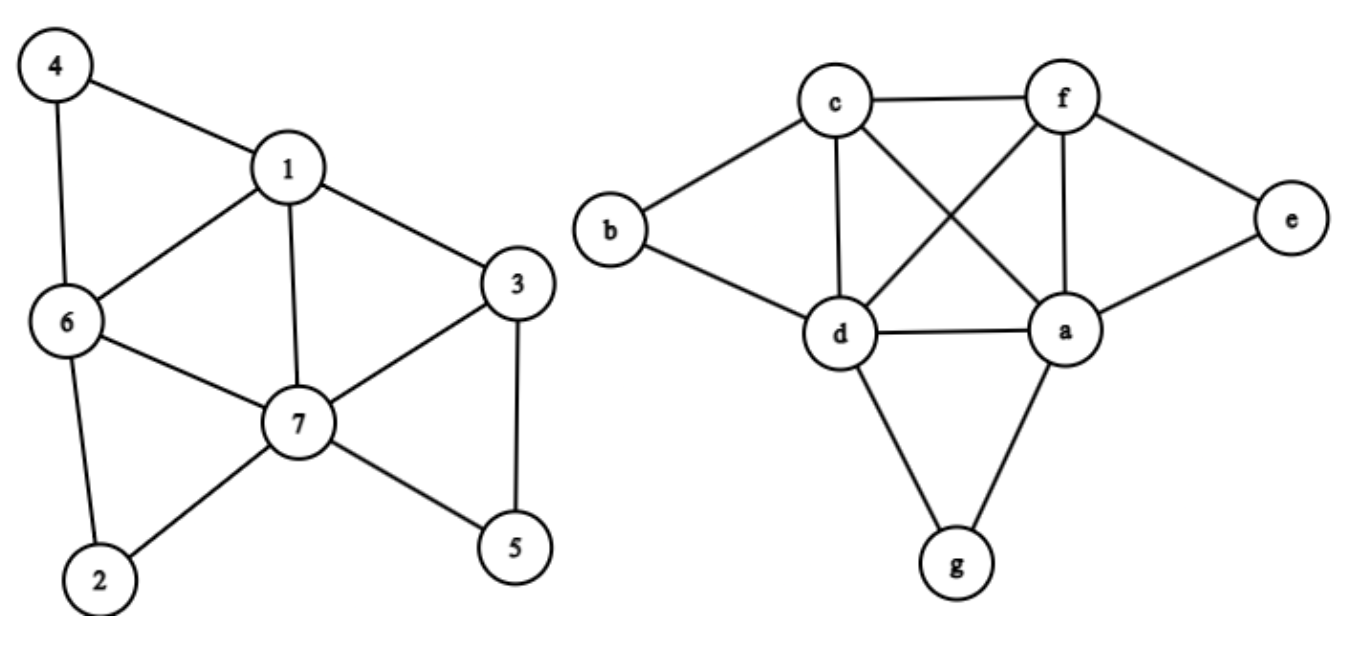
\includegraphics[width=14cm]{images/08-4b.png}
\end{qparts}

\begin{solution}
\end{solution}

\newpage

\subsection*{\probnum Any tours available? [12 points]}
State whether each of the following contains, or is guaranteed to contain a Hamiltonian Cycle. Justify your response for each part. 
\begin{qparts}
    \item ~\\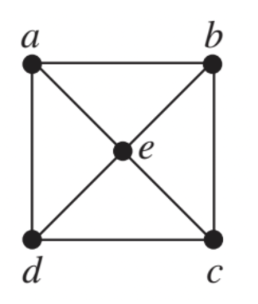
\includegraphics[width=3cm]{images/08-5a.png} 
    \item ~\\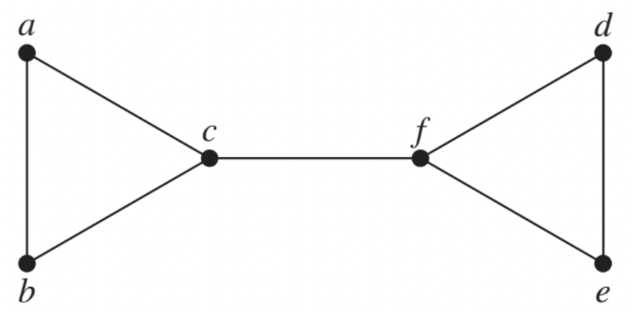
\includegraphics[width=7.5cm]{images/08-5b.png} 
    \item A simple, bipartite graph with 4 vertices that contains one cycle
    \item A 4-vertex graph where each vertex has even degree 
\end{qparts}

\begin{solution}
\end{solution}

\newpage
\subsection*{\probnum Euler Visits the U.S. [12 points]}
Let $G=(V,E)$ be a graph of the continental U.S. where $V$ is the set of the first 48 states (excluding Alaska and Hawaii) and $E$ contains all pairs that share a border.  (Arizona and Colorado do not share a border, nor do Utah and New Mexico). A reference for the U.S. map has been provided below.

\begin{center}
    ~\\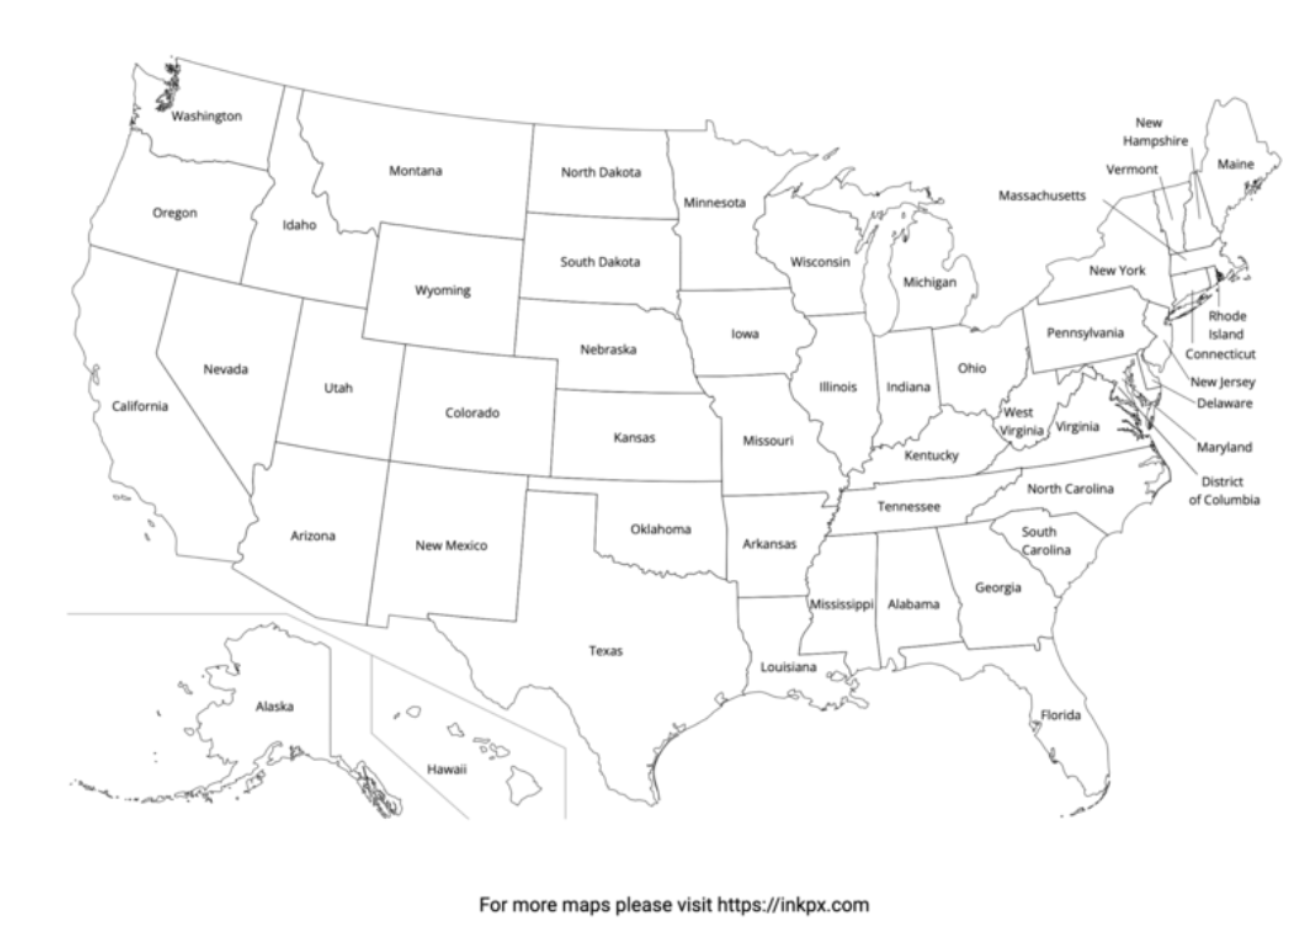
\includegraphics[width=15cm]
    {images/08-6.png}
\end{center}

\begin{qparts}
    \item Does $G$ have an Euler path?  Prove or disprove.
    
    \item Is $G$ 3-colorable?  In other words, is there a function $f\colon V\rightarrow\{\text{red,blue,green}\}$ such that if $\{u,v\}\in E$ then $f(u)\neq f(v)$?

    \textbf{Hint:} Consider odd wheels $W_{2k + 1}$ 
\end{qparts}

\begin{solution}
\end{solution}

\newpage
\subsection*{\probnum Ham and Cheese [15 points]}
A Hamiltonian cycle is a cycle that traverses through every vertex in a graph exactly once (starting and ending at the same vertex). How many Hamiltonian cycles are there in the complete graph $K_n$? Justify your answer.

\textbf{Note:} Two cycles are the same as long as the have the same vertices, and each vertex has the same left and right neighbors in the cycle. For instance the cycles $(a,b,c,a),$ $(b,c,a,b),$ and $(a,c,b,a)$ are all equivalent.

\begin{solution}
\end{solution}

\subsection*{\probnum Captivating Counts [14 points]}
How many positive integers between $1000$ and $9999$ inclusive
\begin{qparts}
    \item have distinct digits?
    \item are divisible by 5 or 7?
    \item are divisible by 5 but not by 7?
\end{qparts}
Justify \textbf{and simplify} your answers. You may use a calculator to simplify.

\begin{solution}
\end{solution}

\pagebreak
\section*{Grading of Groupwork \prevhwnum{}}
Using the solutions and Grading Guidelines, grade your Groupwork \prevhwnum{} Problems:
\begin{itemize}
    \item Use the table below to grade your past groupwork submission and calculate scores.
    \item While grading, mark up your past submission. Include this with the table when you submit your grading.
    \item Write whether your submission achieved each rubric item. If it didn't achieve one, say why not.
    \item For extra credit, write positive comment(s) about your work.
    \item You don't have to redo problems correctly, but it is recommended!
    \item See ``All About Groupwork" on Canvas for more detailed guidance, and what to do if you change groups.
\end{itemize}

\begin{center}
\resizebox{\textwidth}{!}{\begin{tabular}{| c | c | c | c | c | c | c | c | c | c | c | c | c |}
\hline
 & (i) & (ii) & (iii) & (iv) & (v) & (vi) & (vii) & (viii) & (ix) & (x) & (xi) & Total:\\
\hline
Problem 1 & & & & & & &\filcl &\filcl &\filcl & \filcl& \filcl& \hspace{1cm}/10\\
\hline 
Problem 2 & & & & & & &\filcl &\filcl &\filcl & \filcl& \filcl& \hspace{1cm}/8\\
\Xhline{1.25pt}
Total: &\filcl &\filcl &\filcl &\filcl &\filcl &\filcl &\filcl &\filcl & \filcl& \filcl& \filcl&\hspace{1cm}/18\\
\hline
\end{tabular}}
\end{center}

\pagebreak
\setcounter{probnumcount}{1}
\section*{Groupwork \hwnum{} Problems}

\subsection*{\probnum Commit Tea Party [15 points]} 
Two committees are having a meeting. If there are 12 people in each committee, how many different ways can they sit around a table given the following restrictions? Note that two orderings are considered equal if each person has the same two neighbors (without distinguishing their left and right neighbors).

\begin{qparts}
    \item There are no restrictions on seating.
    \item Two people in the same committee cannot be neighbors.
    \item Everybody must have exactly two neighbors from their committee.
    \item Everybody must have exactly one neighbor from their committee.
\end{qparts}

\begin{solution}
\end{solution}

\subsection*{\probnum Hiking Extravaganza [15 points]}
Prove that every complete $n$-node weighted graph (with all possible edges) with $n \ge 1$ and all distinct edge weights has a (possibly non-simple) path of $n-1$ edges along which the edge weights are strictly increasing.

\textbf{Hint:} Start by placing a hiker on each node. Try to show that the hikers can walk paths of \emph{total} length $n(n-1)$, each along increasing-weight paths.

\begin{solution}
\end{solution}

\end{document}

